\section{Geometry}

\subsection{Convex and Concave Polygons}


\begin{figure}[H]
    \centering
    \begin{minipage}[b]{0.25\textwidth}
        \centering
        \includegraphics[width=\linewidth]{media/Convex-Polygon.jpg}
        \caption{Convex Polygon}
    \end{minipage}%
    \begin{minipage}[b]{0.25\textwidth}
        \centering
        \includegraphics[width=\linewidth]{media/Concave-Polygon.jpg}
        \caption{Concave Polygon}
    \end{minipage}
    \caption{Two Types of Polygons}
\end{figure}

\subsubsection{Regular polygon circumradius}

    \def\R{3}

    \begin{figure}[H]
        \centering
        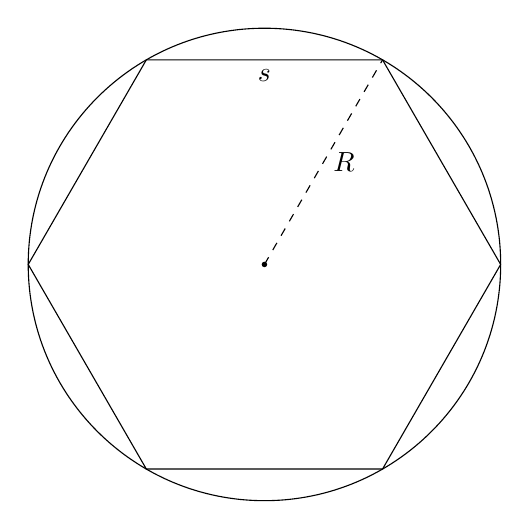
\begin{tikzpicture}
            \draw (0:\R) -- (60:\R) -- node[anchor=north] { $s$ } (120:\R) -- (180:\R) -- (240:\R) -- (300:\R) -- (360:\R) -- (0:\R);
            \draw (0, 0) circle [radius=\R];
            \fill (0, 0) circle [radius=1pt];
            \draw[dashed] (0, 0) -- node[anchor=west] { $R$ } (60:\R);

        \end{tikzpicture}
    \end{figure}

    \[
        R = \frac{s}{2}\csc\frac{\pi}{n}
    \]

\subsubsection{Regular polygon inscribed circle radius}

    \def\R{3}

    \begin{figure}[H]
        \centering
        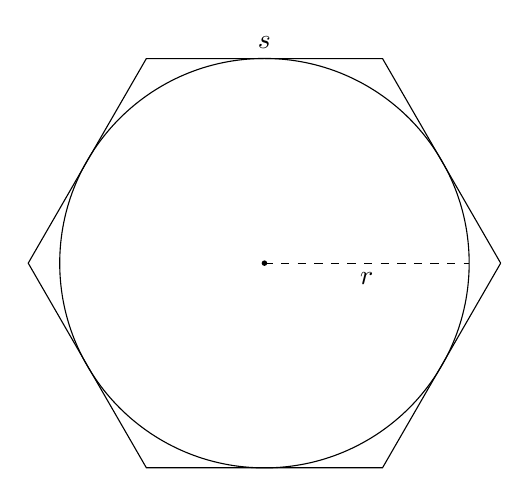
\begin{tikzpicture}
            \draw (0:\R) -- (60:\R) -- node[anchor=south] { $s$ } (120:\R) -- (180:\R) -- (240:\R) -- (300:\R) -- (360:\R) -- (0:\R);
            \draw (0, 0) circle [radius=2.6];
            \fill (0, 0) circle [radius=1pt];
            \draw[dashed] (0, 0) -- node[anchor=north] { $r$ } (2.6, 0);

        \end{tikzpicture}
    \end{figure}

        \[
        r = R\cos \frac{\pi}{n}
        \]



\subsubsection{Area of regular polygons}

    \begin{itemize}
        \item Let $n$ be the number of sides of the regular polygon, the area can be found using one of the values below:
            \begin{enumerate}
                \item  the lenght of one of the sides ($s$)
                \item apothem, the radius of the inscribed circle ($r$)
                \item the radius of the circumscribed circle ($R$)
            \end{enumerate}

        \[
            A = \frac{1}{2}nrs = \frac{1}{4}ns^2\cot \frac{\pi}{n} = nr^2\tan \frac{\pi}{n} = \frac{1}{2}nR^2\sin \frac{2\pi}{n}
        \]

    \end{itemize}


\subsubsection{Sum of internal angle of a regular polygon}
A regular polygon with $n$ sides have $(n-2)180$ degrees as sum of it's internal angle.


\subsection{Trapezium}

\subsubsection{Area}
\begin{figure}
    \centering

    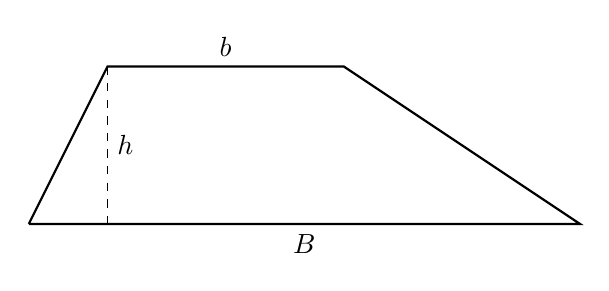
\begin{tikzpicture}
        \coordinate (A) at (0, 0);
        \coordinate (B) at (7, 0);
        \coordinate (C) at (4, 2);
        \coordinate (D) at (1, 2);
        \coordinate (O) at (1, 0);

        \draw[thick] (A) -- node[anchor=north] { $B$ } (B) -- (C) -- node[anchor=south] { $b$ } (D) -- (A);
        \draw[dashed] (D) -- node[anchor=west] { $h$ } (O);

    \end{tikzpicture}
\end{figure}
\[
    A = \frac{(B + b)h}{2}
\]



\subsection{Dot product}
The dot product of vectors $\mathbf{u}$ and $\mathbf{v}$ in $n$ dimensions is given by:
\[
\langle \mathbf{u}, \mathbf{v} \rangle = u_1 \cdot v_1 + u_2 \cdot v_2 + \ldots + u_n \cdot v_n
\]

\subsection{Magnitude}
The magnitude of a vector $\mathbf{v}$ in $n$ dimensions is given by:
\[
|\mathbf{v}| = \sqrt{v_1^2 + v_2^2 + \ldots + v_n^2}
\]

The dot product of two Euclidean vectors $\mathbf{u}$ and $\mathbf{v}$ is defined by

\[
\langle \mathbf{u}, \mathbf{v} \rangle = |\mathbf{u}| \cdot |\mathbf{v}| \cdot \cos(\theta)
\]

\subsection{Equação reduzida da reta}

\begin{equation}
    y = mx + b
\end{equation}

Onde $m$ é o coeficiente angular que representa a taxa de variação da reta: consiste no número de
unidades que $y$ varia para cada unidade de variação de $x$ no sentido positivo do eixo
horizontal. O coeficiente linear $b$ é o valor no qual a reta intercepta o eixo $y$.

Não pode representar retas verticais

\subsection{Equação geral da reta}

\begin{equation}
    ax + by + c = 0
\end{equation}

\subsection{Equação geral da reta a partir de dois pontos}

Seja $P = (x_p, y_p)$ e $Q = (x_p, y_p)$.

$a = y_p - y_q$, $b = x_q-x_p$, $c = x_p y_q - x_q y_p$


\subsection{Inclinação da reta a partir de dois pontos}

Seja $P = (x_p, y_p)$ e $Q = (x_p, y_p)$, a inclinação da reta é dada por:

\begin{equation}
    m = \frac{y_q - y_p}{x_q - x_p}
\end{equation}

\subsection{Pertecimento de ponto a reta}

Seja $r$ uma reta com equação geral $ax + by + c = 0$ e $P = (x_p, y_p) $ um ponto qualquer, $P \in r$ se, e somente se : $a x_p + b x_p + c = 0$

\subsection{Distância entre dois pontos (euclidiana)}

A distância euclidiana entre dois pontos $A = (x_a, y_a)$ e $B = (x_b, y_b)$ é dada por :

$$ \sqrt{(x_a-y_a)^2 + (y_a-y_b)^2} $$

\subsection{Distância entre ponto e reta}

A distância de um ponto $P$ a uma reta $r$ é definida como a menor disância possível entre todos os pontos de $r$ e $P$. A menor distância será aquela entre o ponto $P$ e o ponto de intersecção $Q$ de $r$ com a reta perpendicular a $r$ que passa por $P$.

A distância $d$ entre $P = (x_p, y_p)$ e a reta $ax + by + c = 0$ é dada por :

\begin{equation}
    \frac{|a x_p + b y_p +c|}{\sqrt{a^2+b^2}}
\end{equation}

As coordenadas do ponto $Q$ = $(x_q, y_q)$ sáo dadas por : 

\begin{equation}
x_q = \frac{b (b x_p - a y_p)-ac}{a^2+b^2} \quad \text{, } \quad y_q = \frac{a(-bx_p+ay_p)-bc}{a^2+b^2}
\end{equation}

